\subsection{Expanding around Minimum of Linear $\sigma$-model}

The Lagrangian density
\begin{equation}
    \mathscr{L}=\mathcal{L}_{\text{kin}}-V(\sigma,\vec{\pi})=-\frac{1}{2}(\partial_\mu\sigma)(\partial^\mu\sigma)-\frac{1}{2}(\partial_\mu\vec{\pi})(\partial^\mu\vec{\pi})+\frac{1}{2}\mu^2(\sigma^2+\vec{\pi}^2)+\frac{\lambda}{4}(\sigma^2+\vec{\pi}^2)^2+h\sigma
\end{equation}
can be expanded around the minimum at $\sigma_0=f_\pi+h\cdot\frac{1}{2\mu^2}+\mathcal{O}(h^2)$ where $f_\pi=\frac{\mu}{\sqrt{\lambda}}$. Performing the substitution $\sigma\mapsto v+\sigma$ and neglecting terms of order $\mathcal{O}(h^2,\sigma^3,\sigma\vec{\pi}^2,(\vec{\pi}^2)^2)$ and higher the potential reads
\begin{equation}
    V(\sigma,\vec{\pi})=-\frac{\mu^4}{4\lambda}+\frac{1}{2}m_\sigma\sigma^2+\frac{1}{2}m_\pi^2\vec{\pi}^2
\end{equation}
with pion mass $m_\pi^2=\frac{h}{f_\pi}$ and sigma mass $m_\sigma^2=2\mu^2+\mathcal{O}(h)$. Defining $\pi^\pm=(1/\sqrt{2})(\pi^1\mp\imagu\pi^2)$ one gets 
\begin{equation}
    (\pi^1)^2+(\pi^2)^2=\abs{\pi^+}^2+\abs{\pi^-}^2=2\pi^+\pi^-\equiv 2\pi^+\overline{\pi^+}
\end{equation}

The expansion of the Lagrangian around $\sigma_0$ breaks the $SO(4)$-symmetry associated to the vector $(\sigma,\vec{\pi})$ and chooses explicitly a minimum within the $SO(4)$-symmetric mexican hat potential. The residual symmetry is $SU(3)$. It features the $SO(2)$ subgroup of symmetry transformations
\begin{equation}
    \begin{pmatrix}
        \pi^1\\\pi^2
    \end{pmatrix}
        \mapsto
        \begin{pmatrix}
            \cos\alpha&\sin\alpha\\-\sin\alpha&\cos\alpha
        \end{pmatrix}
        \begin{pmatrix}
            \pi^1\\\pi^2
        \end{pmatrix}
        \qquad\iff\qquad\pi^\pm\mapsto e^{\pm\imagu\alpha}\pi^\pm
\end{equation}
Note $\pi^-=\overline{\pi^+}$.

The Lagrangians and energy-momentum tensors $T^{\mu\nu}=2(\partial\mathscr{L}/\partial g_{\mu\nu})+g^{\mu\nu}\mathscr{L}$ \textbf{CITE: BLAU NOTES} for the separate fields read
\begin{subequations}
    \begin{align}
        \mathscr{L}_{\pi^\pm}&=-(\partial_\mu\pi^+)(\overline{\partial_\mu\pi^+})-m_\pi^2\pi^+\overline{\pi^+}&T^{\mu\nu}_{\pi^\pm}&=2(\partial^\mu\pi^+)(\overline{\partial^\nu\pi^+})+g^{\mu\nu}\big(-(\partial_\alpha\pi^+)(\overline{\partial_\alpha\pi^+})-m_\pi^2\pi^+\overline{\pi^+}\big)\\
        \mathscr{L}_{\pi^0}&=-\frac{1}{2}(\partial_\mu\pi^0)(\partial^\mu\pi^0)-\frac{1}{2}m_\pi^2(\pi^0)^2&T^{\mu\nu}_{\pi^0}&=(\partial^\mu\pi^0)(\partial^\nu\pi^0)+g^{\mu\nu}\big(-\frac{1}{2}(\partial_\alpha\pi^0)(\partial^\alpha\pi^0)-\frac{1}{2}m_\pi^2(\pi^0)^2\big)\\
        \mathscr{L}_\sigma&=-\frac{1}{2}(\partial_\mu\sigma)(\partial^\mu\sigma)-\frac{1}{2}m_\sigma^2\sigma^2&T^{\mu\nu}_{\sigma}&=(\partial^\mu\sigma)(\partial^\nu\sigma)+g^{\mu\nu}\big(-\frac{1}{2}(\partial_\alpha\sigma)(\partial^\alpha\sigma)-\frac{1}{2}m_\pi^2(\pi^0)^2\big)
    \end{align}
\end{subequations}

\subsubsection{Matching to Fluid Variables for the Real Field $\pi^0$}

The only availabe $4$-vector in the fluid theory is $u_\mu$. It is thus intuitive to try to identify the real-valued $4$vector $\partial_\mu\pi^0\sim u_\mu$. Taking the normalization $u_\mu u^\mu=-1$ into account, one finds
\begin{equation}
    u_\mu=\frac{\partial_\mu\pi^0}{\chi}\,,\qquad0<\chi^2\defeq-(\partial_\mu\pi^0)(\partial^\mu\pi^0)
\end{equation}
From the fluid theory, we try to match the energy density of the hypothetical superfluid
\begin{subequations}
    \begin{align}
        \epsilon_{s,\pi^0}=u_\mu u_\nu T^{\mu\nu}_{\pi^0}&=\frac{(\partial_\nu\pi^0)(\partial_\mu\pi^0)}{\chi^2}\Big((\partial^\mu\pi^0)(\partial^\nu\pi^0)+g^{\mu\nu}\big(-\frac{1}{2}(\partial_\alpha\pi^0)(\partial^\alpha\pi^0)-\frac{1}{2}m_\pi^2(\pi^0)^2\big)\Big)\\
        &=\chi^2-\big(\frac{1}{2}\chi^2-\frac{1}{2}m_\pi^2(\pi^0)^2\big)\\
        &=\frac{m_\pi^2(\pi^0)^2+\chi^2}{2}
    \end{align}
\end{subequations}

The equations of motion for the real Klein-Gordon field are
\begin{equation}
    (-\Box+m_\pi^2)\pi^0=0
\end{equation}


\subsubsection{Matching to Fluid Variables for the Complex Fields $\pi^\pm$}

The $U(1)$-symmetry $\pi^\pm\mapsto e^{\pm\imagu\alpha}\pi^\pm$ with infinitesimal transformation $\pi^\pm\mapsto(1\pm\imagu\delta\alpha)\pi^\pm$ generates a conserved Noether current
\begin{subequations}
    \begin{align}
        j^\mu&\sim\frac{\delta\mathscr{L}}{\delta(\partial_\mu\pi^+)}\delta\pi^++\frac{\delta\mathscr{L}}{\delta(\partial_\mu\pi^-)}\delta\pi^-\\
        &\sim\pi^-(\partial^\mu\pi^+)-\pi^+(\partial_\mu\pi^-)\\
        &=\sqrt{n}\big((\partial_\mu\sqrt{n})+\imagu\sqrt{n}(\partial_\mu\theta)\big)-\sqrt{n}\big((\partial_\mu\sqrt{n})-\imagu\sqrt{n}(\partial_\mu\theta)\big)\\
        &=n(\partial_\mu\theta)
    \end{align}
\end{subequations}
with the parametrization $\pi^\pm=\sqrt{n}e^{\pm\imagu\theta}$. The most intuitive matching is now
\begin{equation}
    u^\mu=\frac{\partial_\mu\theta}{\chi}\,,\qquad 0<\chi^2\defeq-(\partial_\mu\theta)(\partial^\mu\theta)
\end{equation}
leading to the energy density
\begin{subequations}
    \begin{align}
        \epsilon_{s,\pi^\pm}=u_\mu u_\nu T^{\mu\nu}_{\pi^\pm}&=\frac{(\partial_\mu\theta)(\partial_\nu\theta)}{\chi^2}\Big(2(\partial^\mu\pi^+)(\partial^\nu\pi^-)+g^{\mu\nu}\big(-(\partial_\alpha\pi^+)(\partial^\alpha\pi^-)-m_\pi^2\pi^+\pi^-\big)\Big)\\
        &=2\frac{[(\partial_\mu\sqrt{n})(\partial^\mu\theta)]^2}{\chi^2}+2n\chi^2-\big(n\chi^2-(\partial_\mu\sqrt{n})(\partial^\mu\sqrt{n})-m_\pi^2n\big)
    \end{align}
\end{subequations}
where the intermediate calculation
\begin{subequations}
    \begin{align}
        (\partial^\mu\pi^+)(\partial^\nu\pi^-)&=\big((\partial^\mu\sqrt{n})+\imagu\sqrt{n}(\partial^\mu\theta)\big)\big((\partial^\nu\sqrt{n})-\imagu\sqrt{n}(\partial^\nu\theta)\big)\\
        &=(\partial^\mu\sqrt{n})(\partial^\nu\sqrt{n})+n(\partial^\mu\theta)(\partial^\nu\theta)+\imagu\big(\sqrt{n}(\partial^\mu\theta)(\partial^\nu\sqrt{n})-\sqrt{n}(\partial^\nu\theta)(\partial^\mu\sqrt{n})\big)
    \end{align}
\end{subequations}
is useful.

Expressing the Lagrangian in terms of $(n,\theta)$ 
\begin{equation}
    \mathscr{L}_{\pi^\pm}=-(\partial_\mu\sqrt{n})(\partial^\mu\sqrt{n})-n(\partial_\mu\theta)(\partial^\mu\theta)-nm_\pi^2
\end{equation}
yields as the corresponding equations of motion
\begin{subequations}
    \begin{align}
        \partial_\mu\Bigg(\frac{\partial\mathscr{L}_{\pi^\pm}}{\partial(\partial_\mu\sqrt{n})}\Bigg)=\frac{\partial\mathscr{L}_{\pi^\pm}}{\partial\sqrt{n}}&:&-2\Box\sqrt{n}&=-2\sqrt{n}\big((\partial_\mu\theta)(\partial^\mu\theta)+m_\pi^2\big)\\
        \partial_\mu\Bigg(\frac{\partial\mathscr{L}_{\pi^\pm}}{\partial(\partial_\mu\theta)}\Bigg)=\frac{\partial\mathscr{L}_{\pi^\pm}}{\partial\theta}&:&\partial_\mu\big(-2n(\partial^\mu\theta)\big)&=0
    \end{align}
\end{subequations}
the second of which encodes the conservation law for the $U(1)$-Noether current.
    
The easiest (and most naive) solution is again $n=\const$ and $\partial_\mu\theta=p_\mu$ with $p_\mu p^\mu=-m_\pi^2$. This would be a solution with only a single momentum mode. This solution implies $u^\mu=\const$ which is generally not satisfied by the given data. Assume therefore the existence of a small perturbation $\partial_\mu\theta=p_\mu+\delta q_\mu$ with $q_\mu p^\mu = 0$. From this, $\chi^2=-(\partial_\mu\theta)(\partial^\mu\theta)=-p_\mu p^\mu-q_\mu q^\mu=m_\pi^2-\delta^2q^2$. To linear order in $\delta$
\begin{equation}
    \partial_\mu\theta=\chi u_\mu=m_\pi u_\mu
\end{equation}
holds true. To expand the equations of motion and allow for non-constant amplitude, assume $n=n_{(0)}+\delta n_{(1)}(x)$ with $n_{(0)}=\const$ ($\sqrt{n}\approx\sqrt{n_{(0)}}+\delta\cdot n_{(1)}/(2\sqrt{n_{(0)}})$). 
\begin{subequations}
    \begin{align}
        \Box\sqrt{n_{(1)}}&=0+\mathcal{O}(\delta^2)\\
        0&=n_{(0)}\partial_\mu q^\mu+q^\mu\partial_\mu n_{(1)}
    \end{align}
\end{subequations}

\subsubsection{Fourier Transform in Adapted Coordinates}

The relevant example is $\Sigma=\{x^\mu\in\mathbb{R}^{(1,3)}\vert (\tau,r)=(\tau(\alpha),r(\alpha))\}$ with $\tau,r$ defined by the coordinate transformation
\begin{equation}
    \left\{\begin{split}
        t&=\tau\cosh\eta\\
        z&=\tau\sinh\eta\\
        x&=r\cos\varphi\\
        y&=r\sin\varphi
    \end{split}\right.
    \qquad\iff\qquad
    \left\{\begin{split}
        \tau&=\sqrt{t^2-z^2}\\
        \eta&=\artanh(z/t)\\
        r&=\sqrt{x^2+y^2}\\
        \varphi&=\arctan(y/x)
    \end{split}\right.
\end{equation}

Let's first evaluate $p_\mu x^\mu$ in the Bjorken coordinate system. Therefore introduce an analogous coordinate change in momentum space
\begin{equation}
    \left\{\begin{split}
        p_t&=m_\perp\cosh\eta_p\\
        p_z&=m_\perp\sinh\eta_p\\
        p_x&=p_\perp\cos\varphi_p\\
        p_y&=p_\perp\sin\varphi_p
    \end{split}\right.
\end{equation}
to rewrite the scalar product as
\begin{equation}
    p_\mu x^\mu\equiv-\tau(p_t\cosh\eta-p_z\sinh\eta)+r(p_x\cos\varphi+p_y\sin\varphi)=-\tau m_\perp\cosh(\eta-\eta_p)+r p_\perp\cos(\varphi-\varphi_p)
\end{equation}
We used the identities
\begin{equation}
    \cosh(a-b)=\cosh a\cosh b-\sinh a\sinh b\,,\qquad\cos(a-b)=\cos a\cos b+\sin a\sin b
\end{equation}
The integral measure changes according to $\dt^4p_{\text{cart}}=\dt m_\perp\dt p_\perp\dt\eta_p\dt\varphi_p\cdot m_\perp p_\perp$. The momentum shell condition $p^2=m^2$ is equivalently parametrized by $m_\perp^2=p_\perp^2+m^2\eqdef \omega_\perp^2$.

\begin{calc}[Metric on Hypersurface]{calc:HypersurfaceMetric}
    Recall the metric $g_{\mu\nu}=\text{diag}(-1,1,\tau^2,r^2)$ in coordinates $(\tau,r,\eta,\varphi)$. Orthonormal tangent vectors to the freeze out hypersurface are $(\hat\partial_\varphi)^\mu=(0,0,0,r^{-1})=r^{-1}(\partial_\varphi)^\mu$, $(\hat\partial_\eta)^\mu=(0,0,\tau^{-1},0)=\tau^{-1}(\partial_\eta)^\mu$ and $(\hat\partial_\alpha)^\mu=\sqrt{r^{\prime 2}(\alpha)-\tau^{\prime 2}(\alpha)}^{-1}(\tau^{\prime}(\alpha),r^{\prime}(\alpha),0,0)=D(\alpha)(\partial_\alpha)^\mu$ with $D(\alpha)=\sqrt{r^{\prime 2}(\alpha)-\tau^{\prime 2}(\alpha)}^{-1}$. The projector on the hypersurface is
    \begin{equation}
        \gamma_{\mu\nu}=(\hat\partial_\varphi)_\mu(\hat\partial_\varphi)_\nu+(\hat\partial_\eta)_\mu(\hat\partial_\eta)_\nu+(\hat\partial_\alpha)_\mu(\hat\partial_\alpha)_\nu=\begin{pmatrix}
            D^2(\alpha)\tau^{\prime2}(\alpha)               & -D^2(\alpha)\tau^\prime(\alpha)r^\prime(\alpha) & 0      & 0   \\
            -D^2(\alpha)\tau^\prime(\alpha)r^\prime(\alpha) & D^2(\alpha)r^{\prime2}(\alpha)                  & 0      & 0   \\
            0                                               & 0                                               & \tau^2 & 0   \\
            0                                               & 0                                               & 0      & r^2
        \end{pmatrix}
    \end{equation}
    The normal of the hypersurface is $n^\mu\equiv(\hat\partial_\alpha^\perp)^\mu=D(\alpha)(r^\prime(\alpha),\tau^\prime(\alpha),0,0)$ and is timelike where $D$ is real. Naturally $\gamma_{\mu\nu}n^\nu=0$. In the basis $(\partial_\alpha,\partial_\eta,\partial_\varphi,n)$ using (in short form)
    \begin{equation}
        (\partial_\alpha)^\nu\gamma_{\mu\nu}(\partial_\alpha)^\mu=\begin{pmatrix}
            \tau^\prime \\r^\prime
        \end{pmatrix}^T\begin{pmatrix}
            -\tau^\prime \\
            r^\prime
        \end{pmatrix}=D^{-2}
    \end{equation}
    the hypersurface metric in coordinates $x^i=(\alpha,\eta,\varphi)$ reads
    \begin{equation}
        \gamma_{ij}=\text{diag}(D^{-2}(\alpha),\tau^2(\alpha),r^2(\alpha))
    \end{equation}
    and the volume element is given by $\dt\Sigma=r(\alpha)\tau(\alpha) D^{-1}(\alpha)\dt\alpha\dt\eta\dt\varphi$. The oriented surface element is \begin{equation}
        \dt\Sigma^\mu=n^\mu\dt\Sigma=r(\alpha)\tau(\alpha)(r^\prime(\alpha),\tau^\prime(\alpha),0,0)\dt\alpha\dt\eta\dt\varphi
    \end{equation}
\end{calc}

\subsection{Properly Considering all Initial Conditions}

Adapt the reasoning in \cite{Amelino-CameliaEtAl_1997}. The idea is to model a non-linear, particle producing interaction process with the inhomogeneous KG equation. After all interactions have decayed and the source has vanished, the particle are effectively free. One can use the true e.o.m. to evolve initial conditions and then, after all interactions have decayed, reconstruct the hypothetical source term and derive particle production from this. For a field with the e.o.m.
\begin{equation}
    (\Box-m^2)\phi(x)=J(x)
\end{equation}
the particle spectrum after the source has vanished is
\begin{equation}
    2\omega_{\vec{p}}\frac{\dt N}{\dt^3\vec{p}}=\frac{1}{(2\pi)^3}\abs{\tilde{J}(\vec{p})}^2
\end{equation}

Use following conventions:
\begin{impt}[Conventions for Fourier Transform]{impt:FourierConvention_PionProdPaper}
    Signature is $(-,+,+,+)$.
    \begin{subequations}
        \begin{align}
            \tilde{f}(p)               & =\int\dt^4x e^{-\imagu px}f(x)                     \\
            \tilde{f}^{(3)}(t,\vec{p}) & =\int\dt^3xe^{-\imagu\vec{p}{\vec{x}}}f(t,\vec{x}) \\
            \tilde{J}(\vec{p})         & =\tilde{J}(p)\vert_{p^0=\omega_{\vec{p}}}
        \end{align}
    \end{subequations}
\end{impt}

The full solution of a KG-field is specified by 2 initial conditions, e.g. $\phi(t,\vec{x})$ and $\dot{\phi}(t,\vec{x})$ for fixed $t$, or equivalently 2 spectral functions $a(p)$, $b(p)$  within the following decomposition:
\begin{subequations}
    \begin{align}
        \phi(t,\vec{x})       & =2\pi\int\frac{\dt^4p}{(2\pi)^4}\delta(p^2-m^2)\Theta(p^0)\big(a(p)e^{\imagu px}+b(p)e^{-\imagu px}\big)                                                                                                          \\
                              & =\int\frac{\dt^3p}{(2\pi)^3}\frac{1}{2\omega_{\vec{p}}}\big(a(\omega_{\vec{p}},\vec{p})e^{-\imagu(\omega_{\vec{p}}t-\vec{p}\vec{x})}+b(\omega_{\vec{p}},\vec{p})e^{\imagu(\omega_{\vec{p}}t-\vec{p}\vec{x})}\big) \\
        \dot{\phi}(t,\vec{x}) & =\int\frac{\dt^3p}{(2\pi)^3}\frac{1}{2}\big(-\imagu a(\omega_{\vec{p}},\vec{p})e^{-\imagu(\omega_{\vec{p}}t-\vec{p}\vec{x})}+\imagu  b(\omega_{\vec{p}},\vec{p})e^{\imagu(\omega_{\vec{p}}t-\vec{p}\vec{x})}\big)
    \end{align}
    From computing the transformations
    \begin{align}
        \tilde{\phi}^{(3)}(t,\vec{p})=\int\dt^3x e^{-\imagu\vec{p}\vec{x}}\phi(t,\vec{x})             & =\int\dt^3xe^{-\imagu\vec{p}\vec{x}}\int\frac{\dt^3q}{(2\pi)^3}\frac{1}{2\omega_{\vec{q}}}\big(a(\omega_{\vec{q}},\vec{q})e^{-\imagu(\omega_{\vec{q}}t-\vec{q}\vec{x})}+b(\omega_{\vec{q}},\vec{q})e^{\imagu(\omega_{\vec{q}}t-\vec{q}\vec{x})}\big) \\
                                                                                                      & =\frac{1}{2\omega_{\vec{p}}}\big(a(\omega_{\vec{p}},\vec{p})e^{-\imagu\omega_{\vec{p}}t}+b(\omega_{\vec{p}},-\vec{p})e^{\imagu\omega_{\vec{p}}t}\big)                                                                                                \\
        \dot{\tilde{\phi}}^{(3)}(t,\vec{p})=\int\dt^3x e^{-\imagu\vec{p}\vec{x}}\dot{\phi}(t,\vec{x}) & =\frac{1}{2}\big(-\imagu a(\omega_{\vec{p}},\vec{p})e^{-\imagu\omega_{\vec{p}}t}+\imagu b(\omega_{\vec{p}},-\vec{p})e^{\imagu\omega_{\vec{p}}t}\big)
    \end{align}
    we can find the inversion of the parametrization
    \begin{align}
        a(\omega_{\vec{p}},\vec{p})e^{-\imagu\omega_{\vec{p}}t} & =\int\dt^3x\big(\omega_{\vec{p}}\phi(t,\vec{x})+\imagu\dot{\phi}(t,\vec{x})\big)e^{-\imagu\vec{p}\vec{x}}                                                                                                                                          \\
                                                                & =\imagu e^{-\imagu\omega_{\vec{p}}t}\int\dt^3x\big(\phi(t,\vec{x})\overset{\leftarrow}{\partial_t}e^{\imagu(\omega_{\vec{p}}t-\vec{p}\vec{x})}-\phi(t,\vec{x})\overset{\rightarrow}{\partial_t}e^{\imagu(\omega_{\vec{p}}t-\vec{p}\vec{x})}\big)   \\
        b(\omega_{\vec{p}},-\vec{p})e^{\imagu\omega_{\vec{p}}t} & =\int\dt^3x\big(\omega_{\vec{p}}\phi(t,\vec{x})-\imagu\dot{\phi}(t,\vec{x})\big)e^{-\imagu\vec{p}\vec{x}}                                                                                                                                          \\
                                                                & =-\imagu e^{\imagu\omega_{\vec{p}}t}\int\dt^3x\big(\phi(t,\vec{x})\overset{\leftarrow}{\partial_t}e^{-\imagu(\omega_{\vec{p}}t+\vec{p}\vec{x})}-\phi(t,\vec{x})\overset{\rightarrow}{\partial_t}e^{-\imagu(\omega_{\vec{p}}t+\vec{p}\vec{x})}\big)
    \end{align}
\end{subequations}

\subsubsection{Invariance of Fourier Transform w.r.t. Deformations of the Hypersurface}
\label{subsec:FourierDeformHypersurface}

Let $\phi_1,\phi_2$ be fields of equal mass evolving according to the KG equation. Then the current
\begin{equation}
    J_\mu[\phi_1,\phi_2]=-\imagu(\phi_1\partial_\mu\phi_2^*-(\partial_\mu\phi_1)\phi_2^*)\eqdef-\imagu\phi_1\overset{\leftrightarrow}{\partial_\mu}\phi_2
\end{equation}
is conserved. Recall Gauß law
\begin{equation}
    \int_\Omega\dt \Omega\nabla_\mu J^\mu=\int_{\partial\Omega}\dt\sigma_\mu J^\mu
\end{equation}
with $\dt\sigma_\mu$ the outwards oriented surface normal of the spacetime volume $\Omega$. The bilinear form
\begin{equation}
    (\phi_1,\phi_2)_\Sigma=\int_\Sigma\dt\Sigma_\mu J^\mu[\phi_1,\phi_2]=-\imagu\int_\Sigma\dt\Sigma_\mu \phi_1\overset{\leftrightarrow}{\partial^\mu}\phi_2^*
\end{equation}
is therefore independent of the choice of (Cauchy) hypersurface $\Sigma$ (if $\partial\Sigma$ is changed, one must carefully check for further contributions in Gauß law).

\debugbox{
    \begin{minipage}{\linewidth}
        \centering
        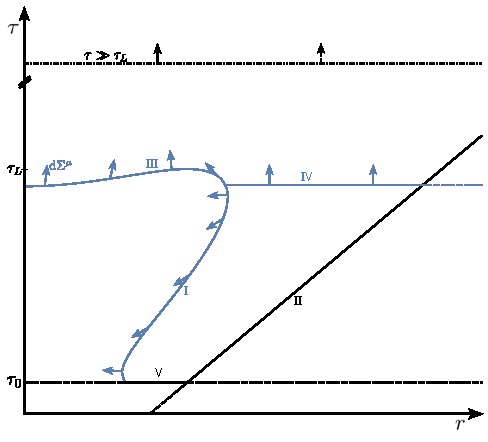
\includegraphics[width=0.4\linewidth]{images/FreezeOutSurface.pdf}
        \captionof{figure}{Freezeout surface in $\tau$-$r$-plane\cite{KirchnerEtAl_2023}.}
        \label{fig:FreezeOutSurface_rtau}
    \end{minipage}
}

Consider the freezeout on the hypersurface depicted in \ref{fig:FreezeOutSurface_rtau}. Assume that the condensate contribution as a function in phase space $f_{\text{cond}}(x^\mu,\vec{p})$ vanishes on $\Sigma_{\text{\rom{2}}}$ and $\Sigma_{\text{\rom{5}}}$, i.e. is contained within the union of all light cones starting on the freeze out surface $\Sigma_{FO}\equiv\Sigma_{\text{\rom{1}}}\cap\Sigma_\text{{\rom{3}}}$. \todo{By causality this seems reasonable, but from Fourier decomposition of a classical field this is not at all clear.}

Following the reasoning from \cite{KirchnerEtAl_2023}, we wish to apply Gauß law. Consider separately the contribution on the $\tau$-axis
\begin{equation*}
    \int_{\Sigma_{r=0}}\dt\Sigma_\mu J^\mu\qquad\text{or}\qquad\lim_{r\to 0}\int_{\Sigma_{r}}\dt\Sigma_\mu J^\mu
\end{equation*}
The surface vector on this hypersurface is $\dt\Sigma_\mu=r\tau\dt\tau\dt\eta\dt\varphi(0,1,0,0)$ and thus vanishes at $r=0$ (the hypersurface $\Sigma_{r=0}$ has zero $3$-volume). Since the derivative in the integrad introduces no divergencies, the contribution of $\Sigma_{r=0}$ to Gauß law is zero.

We can therefore write
\begin{equation}
    \tilde{\phi}(\vec{p})=(\phi,u_{\vec{p}})_{\Sigma_t}=(\phi,u_{\vec{p}})_{\Sigma_{\tau\gg\tau_L}}=(\phi,u_{\vec{p}})_{\Sigma_{FO}}
\end{equation}
The second "$=$" assumes that $\phi=0$ for large spacetime rapidities $\eta\to\pm\infty$ and the $\tau=\const$ hypersurface can be deformed to a $t=\const$ hypersurface.

Note how this has the form of the inner product defined in \ref{subsec:FourierDeformHypersurface}, to be precise
\begin{equation}
    a(\omega_{\vec{p}},\vec{p})=(\phi,e^{-\imagu(\omega_{\vec{p}}t-\vec{p}\vec{x})})_{\Sigma_t}\,,\qquad b(\omega_{\vec{p}},-\vec{p})=-(\phi,e^{\imagu(\omega_{\vec{p}}t-\vec{p}\vec{x})})_{\Sigma_t}
\end{equation}
and can therefore in principle be evaluated on any Cauchy surface.

In \cite{Amelino-CameliaEtAl_1997} it is argued that
\begin{subequations}
    \begin{align}
        \phi_{\text{out}}(t,\vec{p})&=\frac{1}{\omega_{\vec{p}}}\Big([\imagu \tilde{J}(\vec{p})]e^{-\imagu\omega_{\vec{p}}t}-[\imagu \tilde{J}(-\vec{p})]e^{\imagu\omega_{\vec{p}}t}\Big)\\
        \dot{\phi}_{\text{out}}(t,\vec{p})&=\Big(\tilde{J}(\vec{p})e^{-\imagu\omega_{\vec{p}}t}+\tilde{J}(-\vec{p})e^{\imagu\omega_{\vec{p}}t}\Big)
    \end{align}
\end{subequations}
    from which one derives \textbf{\textcolor{red}{prefactor of $2$?}}
\begin{subequations}
    \begin{align}
        \tilde{J}(\vec{p}) & =-\imagu e^{\imagu\omega_{\vec{p}}t}\big(\omega_{\vec{p}} \phi_{\text{out}}(t,\vec{p})+\imagu\dot{\phi}_{\text{out}}(t,\vec{p})\big)                                                                         \\
        \tilde{J}(-\vec{p})&=\imagu e^{-\imagu\omega_{\vec{p}}t}(\omega_{\vec{p}}\phi_{\text{out}}(t,\vec{p})-\imagu\dot{\phi}_{\text{out}}(t,\vec{p}))\\
        \intertext{By substition this gives}
        \tilde{J}(\vec{p}) & =-\imagu e^{\imagu\omega_{\vec{p}}t}\int\dt^3x\big(\omega_{\vec{p}}\phi(t,\vec{x})+\imagu\dot{\phi}(t,\vec{x})\big)e^{-\imagu\vec{p}\vec{x}}                                                                  \\
                           & =\int\dt^3x\big(\phi(t,\vec{x})\overset{\leftarrow}{\partial_t}e^{\imagu(\omega_{\vec{p}}t-\vec{p}\vec{x})}-\phi(t,\vec{x})\overset{\rightarrow}{\partial_t}e^{\imagu(\omega_{\vec{p}}t-\vec{p}\vec{x})}\big)\\
                           \intertext{and}
        \tilde{J}(-\vec{p})&=\imagu e^{-\imagu\omega_{\vec{p}}t}\int\dt^3x\big(\omega_{\vec{p}}\phi(t,\vec{x})-\imagu\dot{\phi}(t,\vec{x})\big)e^{-\imagu\vec{p}\vec{x}}\\
        &=\int\dt^3x\big(\phi(t,\vec{x})\overset{\leftarrow}{\partial_t}e^{-\imagu(\omega_{\vec{p}}t+\vec{p}\vec{x})}-\phi(t,\vec{x})\overset{\rightarrow}{\partial_t}e^{-\imagu(\omega_{\vec{p}}t+\vec{p}\vec{x})}\big)
    \end{align}
\end{subequations}
which, by the same argument as before, is independent of the choice of Cauchy surface. The calculation is the same as before, repeated here for my own clarity (note $\overset{\leftrightarrow}{\partial}=\overset{\leftarrow}{\partial}-\overset{\rightarrow}{\partial}$, unlike before) \textcolor{green}{\textbf{and some errors corrected}}
\begin{subequations}
    \begin{align}
        \tilde{J}(\vec{p}) & =\int_{-\infty}^\infty\dt\eta\int_0^{2\pi}\dt\varphi\int_0^\pi\dt\alpha\tau r\Bigg[\phi(\tau,r)\big(r^\prime\overset{\leftrightarrow}{\partial_\tau}+\tau^\prime\overset{\leftrightarrow}{\partial_r}\big)e^{\imagu(\tau \omega_\perp\cosh(\eta-\eta_p)-r p_\perp\cos(\varphi-\varphi_p))}\Bigg] \\
                           & =\int_{-\infty}^\infty\dt\eta\int_0^{2\pi}\dt\varphi\int_0^\pi\dt\alpha\tau r\Bigg[\phi(\tau,r)\big(r^\prime\overset{\leftrightarrow}{\partial_\tau}+\tau^\prime\overset{\leftrightarrow}{\partial_r}\big)e^{\imagu(\tau \omega_\perp\cosh\eta-r p_\perp\cos\varphi)}\Bigg]                      \\
                           & =\int_0^\pi\dt\alpha\tau r\Bigg[\phi(\tau,r)(r^\prime\overset{\leftrightarrow}{\partial_\tau}+\tau^\prime\overset{\leftrightarrow}{\partial_r})\Big[J_0(r p_\perp)\times\big(-Y_0(\tau\omega_\perp)+\imagu J_0(\tau\omega_\perp)\big)\Big]\Bigg]                                                 \\
                           & =2\pi^2\int_0^\pi\dt\alpha\tau r\Bigg[(r^\prime\partial_\tau+\tau^\prime\partial_r)\phi(\tau,r)\Big[J_0(r p_\perp)\times\big(-Y_0(\tau\omega_\perp)+\imagu J_0(\tau\omega_\perp)\big)\Big]+\nonumber                                                                                             \\
                           & \phantom{=}\qquad + \phi(\tau,r)\Big[\tau^\prime\times p_\perp J_1(r p_\perp)\times\big(-Y_0(\tau\omega_\perp)+\imagu J_0(\tau\omega_\perp)\big)+\nonumber                                                                                                                                       \\
                           & \phantom{=}\qquad\phantom{+\phi(\tau,r)\Big[}+r^\prime\times J_0(r p_\perp)\times\omega_\perp\big(-Y_1(\tau\omega_\perp)+\imagu J_1(\tau\omega_\perp)\big)\Big]\Bigg]
    \end{align}
\end{subequations}

The above logic holds true for real sources. Real fields in the present approach are $(\sigma,\pi^a)$. One should expect that $J_{\pi^\pm}=\frac{1}{\sqrt{2}}(J_{\pi^1}\pm\imagu J_{\pi^2})$.

\begin{subequations}
    \begin{align}
        \pi^\pm&=\frac{1}{\sqrt{2}}(\pi^1\mp\imagu\pi^2)=\sqrt{n}e^{\pm\imagu\theta}&\partial_\mu\pi^\pm&=\pm\imagu(\partial_\mu\theta)\pi^\pm=\pm\imagu\chi u_\mu\pi^\pm\\
        \pi^1&=\sqrt{2}\Re\pi^+&\partial_\mu\pi^1&=\sqrt{2}\chi u_\mu\Re(\imagu\pi^+)=-\sqrt{2}\chi u_\mu\Im\pi^+=\chi u_\mu\pi^2\\
        \pi^2&=-\sqrt{2}\Im\pi^+&\partial_\mu\pi^2&=-\sqrt{2}\chi u_\mu\Im(\imagu\pi^+)=-\sqrt{2}\chi u_\mu\Re\pi^+=-\chi u_\mu\pi^1        
    \end{align}
\end{subequations}

If we consider the $U(1)$-symmetry $\pi^\pm\mapsto\pi^\pm e^{\pm\imagu\theta_0}$, taking the above equalities for $\theta_0=0$ (i.e. $\pi^\pm=\pi^\pm(0)$ etc.), then
\begin{subequations}
    \begin{align}
        \pi^1(\theta_0)&=\sqrt{2}\Re(e^{\imagu\theta_0}\pi^+)=\sqrt{2}(\cos\theta_0\Re\pi^+-\sin\theta_0\Im\pi^+)=\pi^1\cos\theta_0+\pi^2\sin\theta_0\\
        \pi^2(\theta_0)&=-\sqrt{2}\Im(e^{\imagu\theta_0}\pi^+)=-\sqrt{2}(\cos\theta_0\Im\pi^++\sin\theta_0\Re\pi^+)=\pi^2\cos\theta_0-\pi^1\sin\theta_0
    \end{align}
\end{subequations}
The final $\pi^\pm$ spectrum will be given by
\begin{equation}
    2\abs{J_{\pi^\pm}(\theta_0)}^2=\abs{J_{\pi^1}(\theta_0)\mp\imagu J_{\pi^2}(\theta_0)}^2=\abs{\cos\theta_0J_{\pi^1}+\sin\theta_0J_{\pi^2}\mp\imagu(J_\pi^2\cos\theta_0-J_{\pi^1}\sin\theta_0)}^2=\abs{(J_{\pi^1}\mp\imagu J_{\pi^2})e^{\pm\imagu\theta_0}}^2
\end{equation}